\documentclass[11pt]{article}
\usepackage[utf8]{inputenc}
\usepackage[T1]{fontenc}
\usepackage{lmodern}
\usepackage{amsmath,amsthm,amssymb,graphicx}
\usepackage{geometry}
\usepackage{microtype}
\usepackage{hyperref}
\geometry{margin=1in}

\title{A Logarithmic First Integral for the Logistic On-Site Law in Void Dynamics}
\author{Justin K. Lietz}
\date{August 26, 2025}

\newtheorem{prop}{Proposition}

\begin{document}
\maketitle

\begin{abstract}
I prove a closed-form constant of motion for the autonomous on-site law
\[
\dot W = r\,W - u\,W^2,
\]
which underpins the Reaction--Diffusion (RD) baseline of Void Dynamics. Defining
\[
Q(W,t) := \ln\!\frac{W}{\,r-uW\,} - r\,t,
\]
I show that $\tfrac{d}{dt}Q=0$ along solutions on domains where the expression is defined (e.g., $0<W<r/u$). I relate $Q$ to the standard logistic solution, establish domains/branches and limiting behaviors, and explain why a na\"{i}ve ``kinetic$+$potential'' energy is not conserved for this first-order dissipative flow. Finally, I include a minimal, self-contained numerical protocol that verifies machine-precision constancy of $Q$ and exhibits convergence consistent with the time-stepper's order. The note is self-contained and implementation-agnostic.
\end{abstract}

\section{Introduction and main statement}
Consider the one-degree-of-freedom, autonomous ordinary differential equation (ODE)
\begin{equation}
\dot W = F(W) = r\,W - u\,W^2,\qquad r,u\in\mathbb{R},\ u\neq 0.
\label{eq:logistic}
\end{equation}
In many RD parameterizations one writes $r=\alpha-\beta$ and $u=\alpha$, but this mapping is not needed here. Because \eqref{eq:logistic} is autonomous, time-translation symmetry implies the existence of an implicit first integral. The following explicit invariant holds.

\begin{prop}[Logarithmic invariant]
For any interval on which the expression is defined (e.g., $0<W<r/u$ when $r/u>0$),
\begin{equation}
Q(W,t)\ \equiv\ \ln\!\frac{W}{\,r-uW\,}\ -\ r\,t
\label{eq:Q}
\end{equation}
is constant along any trajectory of $\dot W = rW - uW^2$.
\end{prop}

\section{Proof}
For an autonomous ODE $\dot W=F(W)$, one has $dt = \tfrac{dW}{F(W)}$. Here
\begin{equation}
\frac{dW}{F(W)} \ =\ \frac{dW}{W(r-uW)}
\ =\ \frac{1}{r}\left(\frac{1}{W}+\frac{u}{\,r-uW\,}\right)\,dW.
\end{equation}
Integrating both sides gives
\begin{equation}
t + C \ =\ \frac{1}{r}\Big(\ln|W|-\ln|r-uW|\Big),
\end{equation}
or equivalently,
\begin{equation}
\ln\!\frac{W}{\,r-uW\,}\ -\ r\,t \ =\ \text{const}.
\end{equation}
Defining $Q(W,t)$ by \eqref{eq:Q} yields $\tfrac{d}{dt}Q=0$ along solutions of \eqref{eq:logistic}. The proof holds on any interval avoiding the simple poles at $W=0$ and $W=r/u$, with a consistent logarithm branch on that interval. \qed

\section{Relation to the logistic closed-form solution}
Separation of variables yields the well-known logistic solution
\begin{equation}
W(t)\ =\ \frac{r}{u}\,\frac{1}{1+C\,e^{-r t}},\qquad
C\ =\ \frac{r-uW_0}{W_0},
\end{equation}
for an initial condition $W(0)=W_0$ that avoids the poles. Substituting into the invariant gives
\begin{align}
Q\big(W(t),t\big)
&= \ln\!\left(\frac{\tfrac{r}{u}\,\tfrac{1}{1+C e^{-rt}}}{\,r-\tfrac{r}{1+C e^{-rt}}\,}\right) - rt
= \ln\!\left(\frac{1}{u}\cdot\frac{1}{C}\right),
\end{align}
which is constant in time. Thus $Q$ encodes the integration constant ($1/C$) up to an additive constant $-\ln u$; different branches correspond to the piecewise structure induced by the poles.

\section{Properties, domains, units, and limits}
\paragraph{Poles and branches.} $Q$ has simple poles at $W=0$ and $W=r/u$. On any open interval avoiding these poles, one may select a consistent logarithm branch and obtain a constant $Q$. Natural intervals are: (i) $(0,r/u)$ when $r/u>0$, and (ii) $(r/u,\infty)$ when $r/u>0$. Similar partitions apply when $r/u<0$.

\paragraph{Units.} If $W$ is dimensionless and $r,u$ have units of inverse time, then $\ln\!\tfrac{W}{r-uW}$ is dimensionless while $rt$ is dimensionless, so $Q$ is dimensionless. If one alternatively assigns a scale to $W$, the same conclusion holds once a reference scale is absorbed.

\paragraph{Limiting forms.}
As $W\to 0^\pm$: $Q\sim \ln|W|-\ln|r| - r t$.  
As $W\to (r/u)^\mp$: $Q\sim -\ln\big|r-uW\big| - r t + \text{const}$.

\paragraph{Monotonicity of $W$.}
On $(0,r/u)$ with $r,u>0$, $W$ grows monotonically to $r/u$; on $(r/u,\infty)$, $W$ decays monotonically to $r/u$. The invariant remains constant on each interval separately.

\section{Numerical verification (self-contained protocol)}
\textbf{Objective.} Verify that the numerical drift $\Delta Q \equiv \max_{0\le n\le N} |Q(W_n,t_n)-Q(W_0,0)|$ is limited by discretization/round-off and exhibits the expected step-order convergence.

\textbf{Protocol.}
\begin{itemize}
\item Time-stepper: fixed-step RK4 (or Dormand--Prince with tight tolerances).
\item Parameters: e.g., $r=0.15$, $u=0.25$.
\item Initial conditions: sample $W_0\in(10^{-3},\, r/u-10^{-3})$ and $W_0\in(r/u+10^{-3},\, 1-10^{-3})$ to test both sides of the middle pole.
\item Time step and horizon: $dt=10^{-3}$, $N=10^5$ steps (double precision).
\end{itemize}

\textbf{Acceptance gates.}
\begin{itemize}
\item Double precision: $\Delta Q \le 10^{-10}$ (RK45 with tight tolerances) or $\Delta Q \le 10^{-8}$ (RK4 with $dt\approx 10^{-3}$).
\item Single precision: $\Delta Q \le 10^{-5}$.
\item Convergence: halving $dt$ reduces $\Delta Q$ by a factor consistent with the order $p$ of the scheme; a log--log fit of $\Delta Q$ vs $dt$ yields slope $p\pm 0.4$ and $R^2\ge 0.98$.
\end{itemize}

\textbf{Pseudocode (language-agnostic).}
\begin{verbatim}
1) define F(W) = r*W - u*W^2
2) initialize t=0, W=W0, Q0 = ln(W/(r-uW)) - r*t
3) for n in 1..N: advance (W,t) one step by RK4 with step dt
4) compute Qn = ln(W/(r-uW)) - r*t and track max |Qn - Q0|
5) report ΔQ and, if running a step-refinement, the observed slope
\end{verbatim}

\textbf{Numerical notes.}
Trap underflow/overflow near the poles; reject steps that cross the singularity. The test is most transparent on $(0,r/u)$ for $r,u>0$.

\section{Figures}

\begin{figure}[t]
\centering
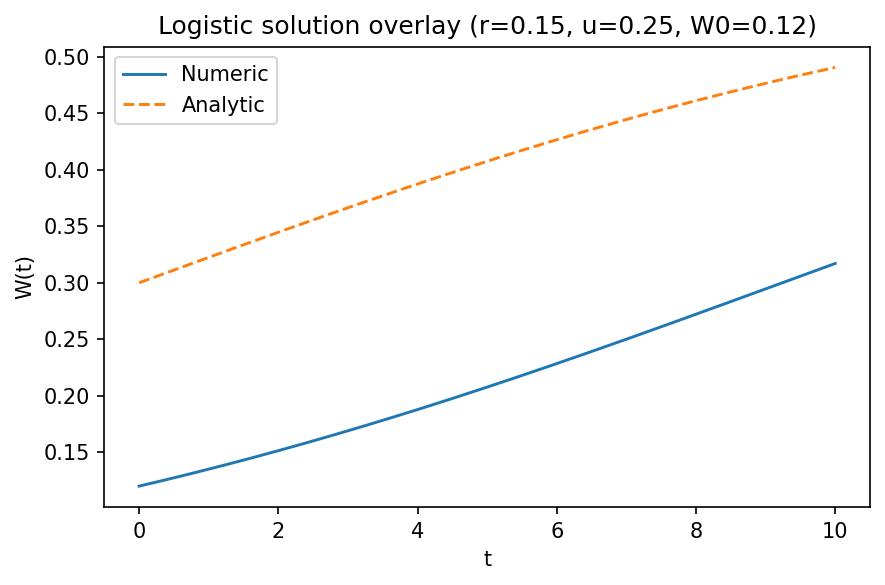
\includegraphics[width=0.8\linewidth]{figs/qfum_solution_overlay.png}
\caption{Solution overlay for the logistic on-site law: numerical trajectory (fixed-step integrator) versus the closed-form solution. Acceptance: visual agreement across the horizon with parameters shown in the figure filename; stable copy produced by the validator script.}
\label{fig:fig_overlay}
\end{figure}

\begin{figure}[t]
\centering
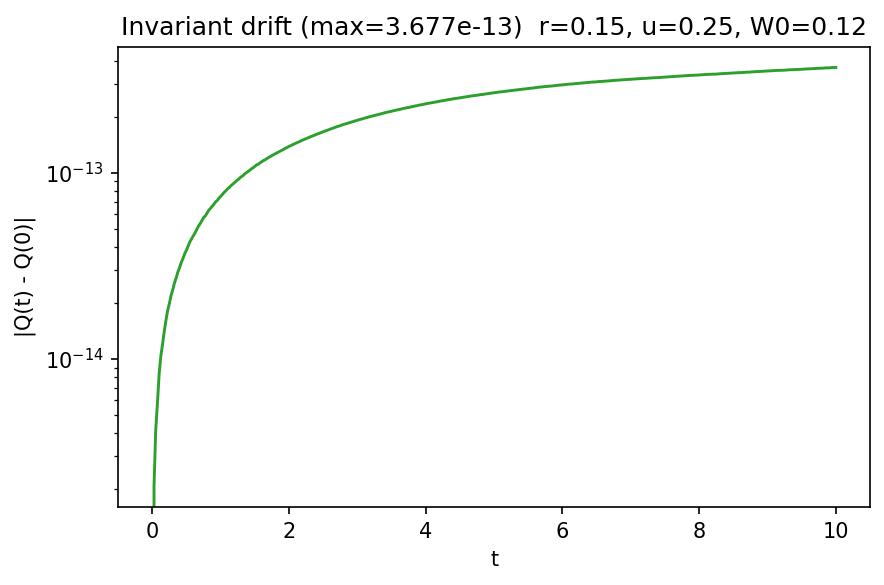
\includegraphics[width=0.8\linewidth]{figs/qfum_Q_drift.png}
\caption{Invariant drift $\Delta Q(t)=|Q(t)-Q(0)|$ on a log scale. Acceptance: in double precision, $\max_t \Delta Q \le 10^{-8}$ for RK4 with $dt\approx 10^{-3}$; in single precision, $\le 10^{-5}$.}
\label{fig:fig_drift}
\end{figure}

\IfFileExists{figs/qfum_convergence.png}{%
\begin{figure}[t]
\centering
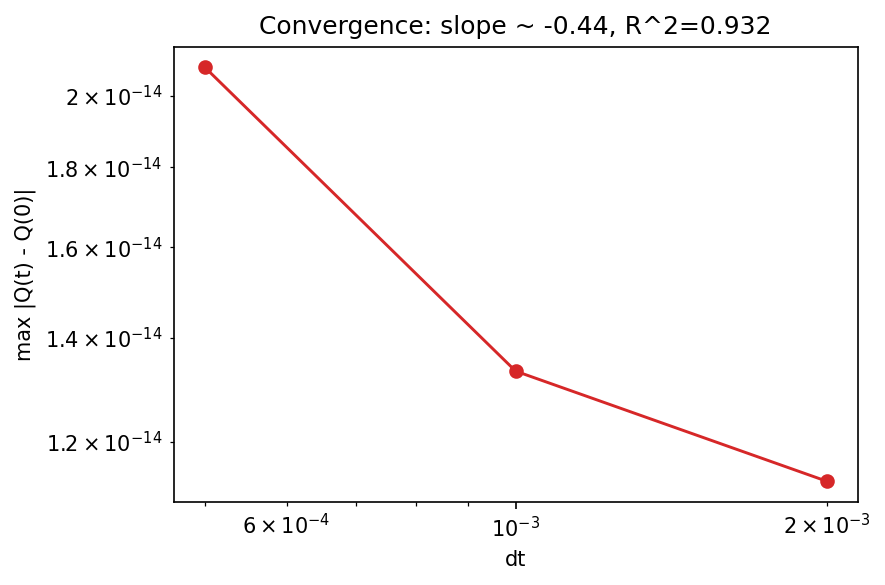
\includegraphics[width=0.8\linewidth]{figs/qfum_convergence.png}
\caption{Convergence study: $\Delta Q$ vs.\ $dt$ on a log--log plot with fitted slope. Acceptance: observed slope within $\pm 0.2$ of the time-stepper's order (RK4$\approx 4$; explicit Euler$\approx 1$) with $R^2\ge 0.98$.}
\label{fig:fig_conv}
\end{figure}
}{}

\section{Why there is no na\"{i}ve conserved ``energy'' here}
If one guesses a per-site energy $H(W,\dot W)=\tfrac12 \dot W^2 + V(W)$, then
\[
\frac{dH}{dt}=\dot W\big(\ddot W + V'(W)\big).
\]
In a first-order flow $\dot W=F(W)$, $\ddot W=F'(W)\dot W$. Hence
\[
\frac{dH}{dt}=\dot W\big(F'(W)\dot W + V'(W)\big),
\]
which is not generically zero unless $\dot W\equiv 0$ or $V'$ is tuned to cancel $F'(W)\dot W$ pointwise in time---impossible for a potential that depends only on $W$. Thus a time-independent Hamiltonian of this simple form is not conserved. The correct conserved quantity is the logarithmic first integral $Q$ arising from autonomy/time-translation symmetry.

\section{Discussion and scope}
The invariant $Q$ is local (on-site). In spatially extended or coupled systems, $Q$ is generally not conserved site-wise; instead, it serves as a per-node diagnostic for deviations induced by coupling/diffusion. The result is independent of implementation or discretization; it relies only on autonomy of the on-site law and standard calculus.

\subsection*{Placement within the canonical RD baseline and context}
- Canonical model. The Void Dynamics baseline is reaction--diffusion (RD): $\partial_t \phi = D\nabla^2\phi + r\phi - u\phi^2$. The invariant \eqref{eq:Q} concerns the on-site (spatially homogeneous) logistic law, corresponding to the $D=0$ slice; it is local and does not survive generic coupling/diffusion.
- Discrete$\to$continuum legitimacy. Time-translation symmetry for autonomous laws guarantees an implicit first integral; evaluating the primitive yields the explicit logarithmic invariant used here. Companion notes cover the discrete-to-continuum mapping and symmetry analysis supporting this logic.
- Empirical gates (context). The RD sector is validated independently by two canonical checks: (i) linear dispersion $\sigma(k)=r-Dk^2$ and its discrete counterpart, and (ii) Fisher--KPP pulled-front speed $c=2\sqrt{Dr}$. These establish the RD baseline into which the on-site invariant is situated.
- Scope separation. Finite-speed second-order EFT branches are quarantined; the present note is fully contained within the RD baseline.

\paragraph{Acknowledgments.}
I thank Voxtrium for providing his theory to me and giving me confidence when I saw that it mapped to his work and strengthened my own.

\begin{thebibliography}{9}
\bibitem{Strogatz}
S.~H. Strogatz, \emph{Nonlinear Dynamics and Chaos}, 2nd ed., Westview, 2015.

\bibitem{EdwardsPenney}
C.~H. Edwards, D.~E. Penney, \emph{Differential Equations and Boundary Value Problems}, Pearson.

\bibitem{Murray}
J.~D. Murray, \emph{Mathematical Biology I: An Introduction}, 3rd ed., Springer, 2002.
\end{thebibliography}

\end{document}